\title{Midterm 1 for Algebra-Based Physics-1: Mechanics (PHYS135A-01)}
\author{Dr. Jordan Hanson - Whittier College Dept. of Physics and Astronomy}
\date{September 25th, 2017}
\documentclass[10pt]{article}
\usepackage[a4paper, total={18cm, 27cm}]{geometry}
\usepackage{outlines}
\usepackage[sfdefault]{FiraSans}
\usepackage{graphicx}

\begin{document}
\maketitle

\section{Estimation, Approximation, and Unit Analysis}
\begin{enumerate}
\item There is a jar full of candies.  Estimate the number of candies in the jar, if this type of round candy has a radius of $\approx 0.3$ cm, and the jar has a radius of $\approx 12$ cm, and a similar height.  (Remember, the answer only has to be accurate to the correct order of magnitude). \vspace{1.5 cm}
\item An explorer lands on Mars, which has an acceleration due to gravity of $\approx 0.4 g$.  If the explorer drops a bag from shoulder height, how long does it take to reach the ground? \vspace{1.5 cm}
\item Our bodies contain special nerve fibers from the spinal cord to extermities, for quick reactions.  Suppose a curious child, who is 0.75 m tall, touches a flame.  The child's body jerks the hand away after 20 milliseconds (0.02 seconds).  What was the speed of the nerve signal? \\
\begin{itemize}
\item A: 1 m
\item B: 5 s
\item C: 20 m/s
\item D: 100 m/s
\end{itemize}
\end{enumerate}
\section{Displacement, Velocity, and Constant Acceleration Vectors}
\begin{enumerate}
\item In the film \textit{The Hunt for Red October}, one scene depicts two Soviet officers at the helm of a submarine they are navigating through an undersea canyon.  Their current speed is 30 kilometers per hour, and the canyon turns 45 degrees to their right 1 kilometer ahead.  In how many seconds must they order the ship to turn before crashing into the side of the canyon?  After the turn, they adjust the speed to 20 kilometers per hour, and travel for 100 seconds.  What is the displacement vector from the original position?\vspace{3cm}
\item A torpedo is dropped in the water 1 km behind the \textit{Red October} by an overflying aircraft, and it accelerates at 3 m/s$^2$, with an initial velocity of 5 m/s.  If the \textit{Red October} does not alter course, but continues at 5 m/s, when will the torpedo reach it?\vspace{3cm}
\end{enumerate}
\section{Vectors}
\begin{enumerate}
\item The astromomer Clyde Tombaugh discovered the pseudo-planet Pluto in 1930.  He observed a section of the night sky and observing the same sky one week later.  He blinked back and forth between images.  A faint star moved across the image.  Knowing how far away stars are, he concluded that the object must be inside our solar system, to be moving at a reasonable velocity.  Thus, it had to be some kind of planet.
\begin{figure}
\centering
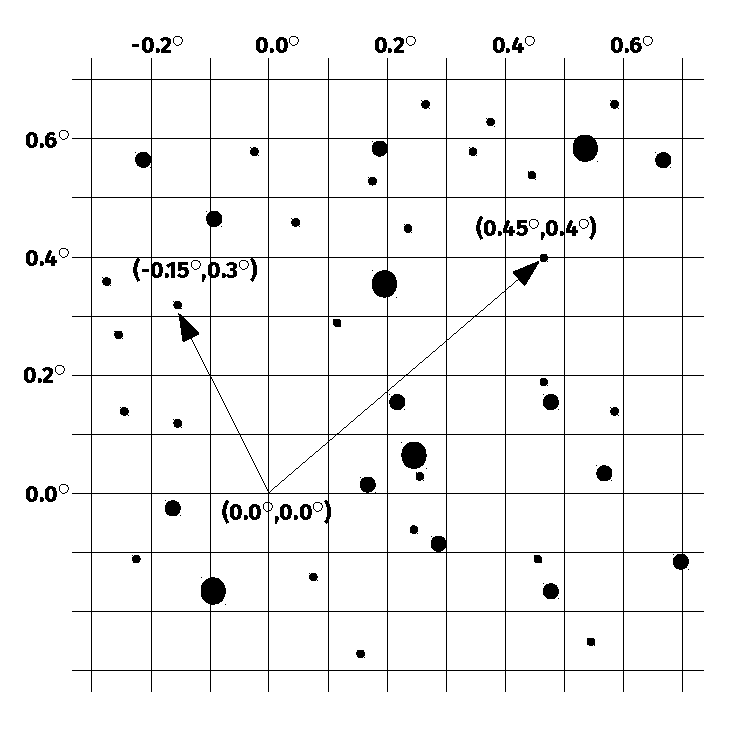
\includegraphics[width=0.5\textwidth]{PlutoDrawing.pdf}
\caption{\label{fig:1} Positions of some unknown celestial body in the solar system, circa 1930.  The vector $(-0.15^{\circ},0.3^{\circ})$ corresponds to the first observation, and the vector $(0.45^{\circ},0.4^{\circ})$ corresponds to the second observation.}
\end{figure}
a) Observe Fig. \ref{fig:1}.  Construct the displacement vector of this object, in units of degrees.  b) Construct the average velocity of this object, in units of degrees per day.  c) Let $s$ be the actual distance traveled, $\theta$ be the observed angle change \textit{in degrees}, and 1AU be the astronomical unit.  At the orbital radius of Pluto, $s[AU] \approx (0.02) \theta[deg]$.  How far in AU did the object move?  d) What is the average velocity from part c) in AU per day?  Does this answer make sense if the object is outside the solar system?
\end{enumerate}
\end{document}
